\documentclass ../main.tex]{subfiles}

\begin{document}



\vspace{3cm}
\chapter{Nociones Previas}

En el estudio de partículas elementales, notamos que experimentalmente se observan efectos tanto cuanticos como relativistas fenomenologicamente. Por lo que para trabajar con ellas se deberá tener en cuenta tanto la mécanica cuántica como la relatividad especial. La teoría con la que más nos acomodará trabajar será la \textbf{Teoría Cuantica de Campos (QFT)} pues tomará ambos efectos en consideración y nos permitirá estudiar eventos que sucedan a velocidades comparables con la velocidad de la luz $c$ en regiones pequeñas.\\

\begin{figure}[h] % "h" intenta colocar la imagen aquí
    \centering
    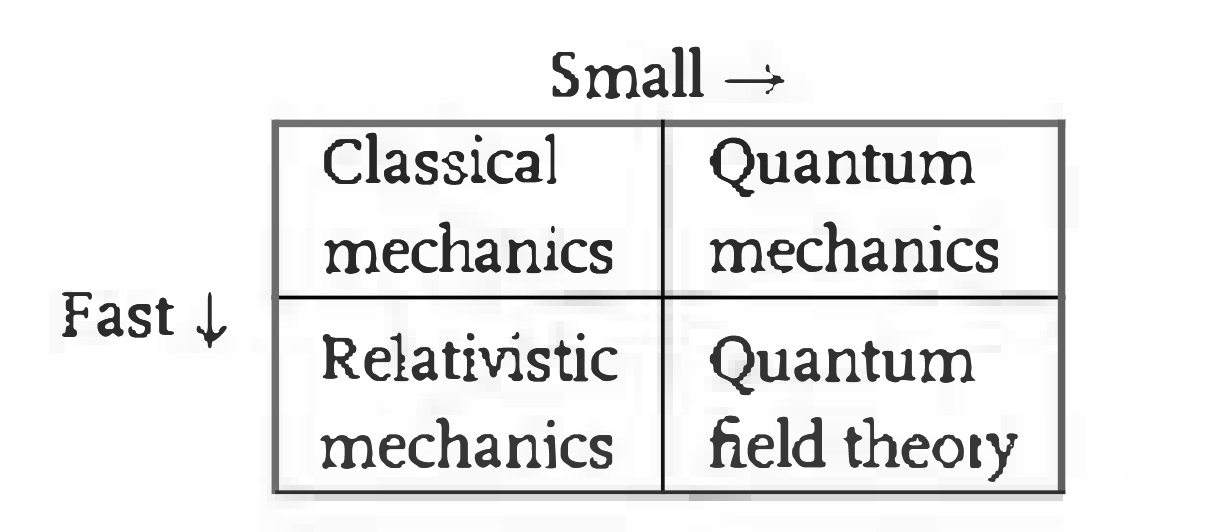
\includegraphics[width=0.5\textwidth]{img/Captura de pantalla 2025-03-29 000744.png}
    \label{fig:graf_QFT}
\end{figure}


Es por esto que para poder estudiar QFT se deberán tener nociones tanto de mécanica clásica como cuántica. En este apunte, no se considerarán los efectos del campo gravitacional. Como las interacciones a estudiar ocurren en regiones pequeñas, el efecto gravitacional será considerado despreciable. 



\section{Primera clase}

\subsection{Derivación de las Ecuaciones de Euler-Lagrange}




\end{document}
